\section{Results}
\label{sec:results}

\subsection{AI model cards}

The level of documentation varies greatly from model to model. We have set up an
automatic documentation system for models trained within \Gls{WIPP}.

\subsection{WIPP 2-steps workflow}

The WIPP 2-steps workflow is first, do the inference of the model and then
compute the accuracy.

\begin{figure}[H]
  \centering
  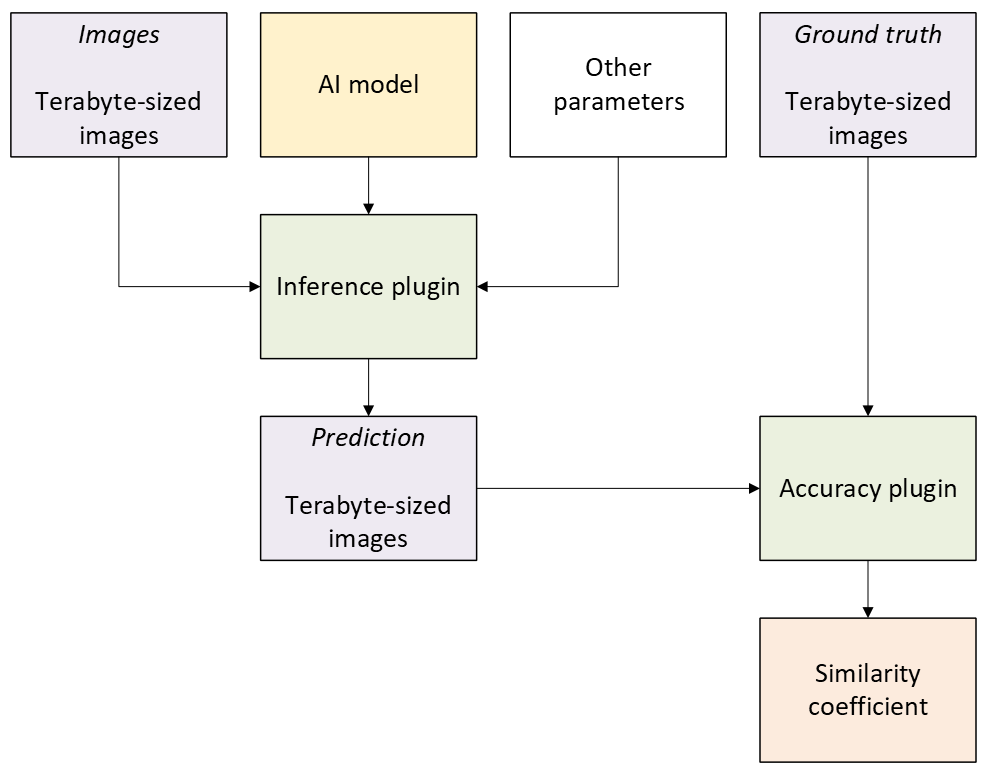
\includegraphics[width=1.0\linewidth]{png/workflow.png}
  \caption{WIPP 2-steps workflow}
  \label{fig:workflow}
\end{figure}

We compute everything in \Gls{WIPP}. The \Gls{WIPP} server specifications are:
\begin{itemize}
  \item CPU: AMD Ryzen 9 3950X 16-Core Processor with 16 cores and 2 threads
  \item GPU: NVIDIA GeForce RTX 3090
  \item 64G RAM
\end{itemize}

\subsection{Dataset 'cell boundary'}

TODO

\subsection{Benchmark 'cell boundary'}

TODO

\subsection{Dataset 'nuclei segmentation'}

TODO

\subsection{Benchmark 'nuclei segmentation'}


TODO

\subsection{Notes}

Even if the results may not be perfect, this method allows you to quickly try
out a new model at reduced cost. It is also easy to change dataset. We can then
take a promising model and improve it by finetuning it. We hope to improve the
speed of data analysis within \Gls{WIPP} and enable better overall results.
